\subsection{Data Collection}
We obtained hourly closing price data for BTC-USD and ETH-USD from January 1, 2023, to October 1, 2024, using the yfinance API.

\subsection{GARCH Modeling}
\label{sec:return_normolize}

% \subsubsection{Mathematical Formulations for GARCH}
% We present the mathematical formulations for GARCH, EGARCH, GJR-GARCH, and others, explaining how each model captures volatility and asymmetry.

\subsubsection{Distribution Choice}
We conducted a series of distributional tests (see Table ~\ref{tab:test_results}) to determine the return distributions. To exclude heteroskedastic factors, we evaluated the distribution of \(\zeta_t := \frac{R_t}{\sigma_t}\), utilizing the Shapiro-Wilk and Kolmogorov-Smirnov tests. Our analysis aimed to validate the assumption of normality for GARCH modeling. The plots in Figures~\ref{fig:normal} and~\ref{fig:qq} represent \(\zeta_t\) calculated from ETH-USD data.

\begin{figure}[ht]
    \centering
    \begin{minipage}{0.5\textwidth}
        \centering
        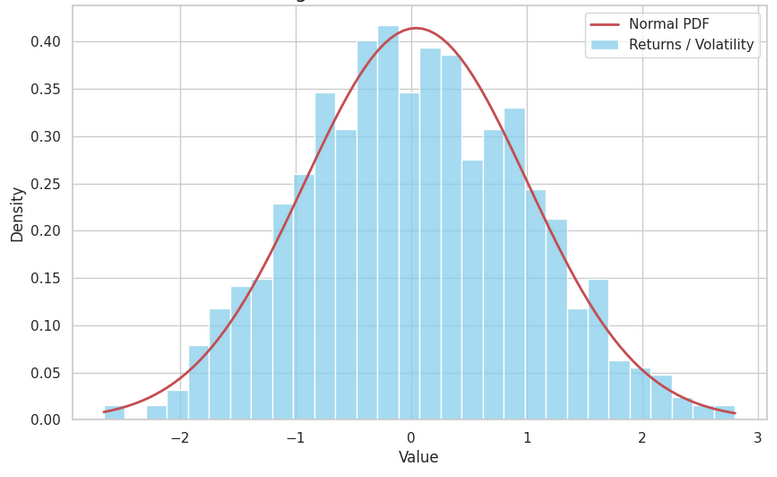
\includegraphics[width=\linewidth]{img/normal.png} % Replace with your image path
        \caption{Normal PDF vs. \(\zeta_t\)}
        \label{fig:normal}
    \end{minipage}
    \hfill
    \begin{minipage}{0.44\textwidth}
        \centering
        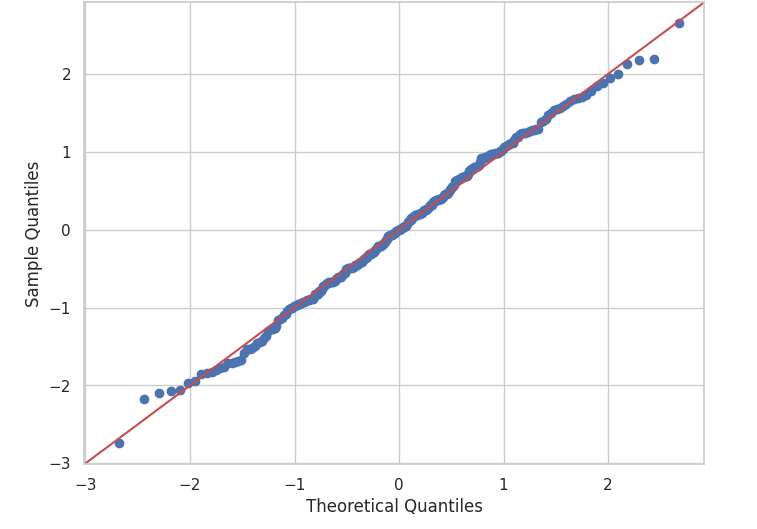
\includegraphics[width=\linewidth]{img/qq.png} % Replace with your image path
        \caption{QQ-Plot of \(\zeta_t\)}
        \label{fig:qq}
    \end{minipage}
\end{figure}

\begin{table}[ht]
\centering
\begin{tabular}{|l|cc|cc|}
\hline
\textbf{} & \multicolumn{2}{c|}{\textbf{Shapiro-Wilk Test}} & \multicolumn{2}{c|}{\textbf{Kolmogorov-Smirnov Test}} \\
\textbf{} & \textbf{Statistic} & \textbf{p-value} & \textbf{Statistic} & \textbf{p-value} \\
\hline
\textbf{BTC-USD} & 0.992 & 0.153 & 0.049 & 0.5214 \\
\hline
\textbf{ETH-USD} & 0.995 & 0.5781 & 0.036 & 0.863 \\
\hline
\end{tabular}
\caption{Statistical Tests Results for BTC-USD and ETH-USD}
\label{tab:test_results}

\end{table}


\subsubsection{Building GARCH Predictions}
The GARCH model directly predicts the current volatility, represented as follows:

\begin{equation}
    \hat{\sigma}_t^2 = \omega + \sum_{i=1}^{q} \alpha_i u_{t-1}^2 + \sum_{j=1}^{p} \beta_j \tilde{\sigma}_{t-j}^2
\end{equation}

Here, \(\tilde{\sigma}_t^2\) denotes the conditional volatility at time \(t\).

In order to prevent data leaks, the final predction of model was obtained in the expanding window style: model was fitted on data from the moment $t=0$ to the moment $t-1$ and then made estimation $\hat{\sigma}_t$. The result of such process can be witnessed at the Figure~\ref{fig:predictions}.

\begin{figure}[ht]
    \centering
    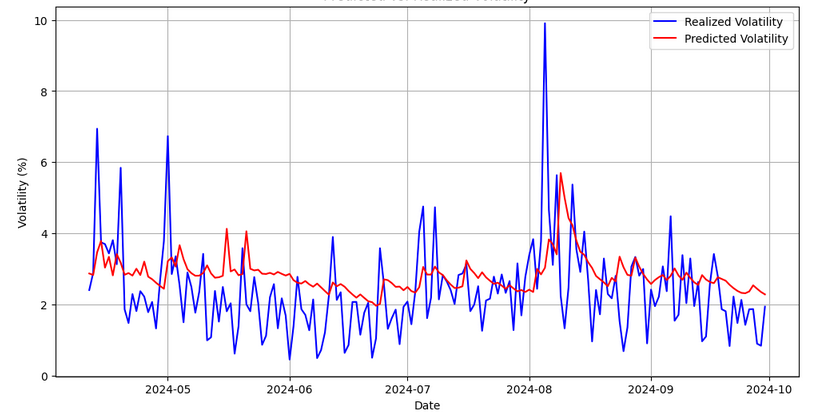
\includegraphics[width=0.7\textwidth]{img/realized_vs_pred.png}  % Adjust width to fit the page
    \caption{Results of GARCH(1,1) Predictions}
    \label{fig:predictions}
\end{figure}

\subsection{Evaluation}
In order to estimate model performance, we computed Mean Squared Error (MSE) and Mean Absolute Error (MAE) of realized volatility values $\sigma_t$ (i.e., ground truth) and GARCH predctions $\hat{\sigma}_t$.

\begin{equation}
    \textsc{MSE}(\{\sigma_t\}_{t=1}^T, \{\hat{\sigma}_t\}_{t=1}^T) := \frac{1}{T}\sum_{t=1}^T (\sigma_t - \hat{\sigma}_t)^2
\end{equation}

\begin{equation}
    \textsc{MAE}(\{\sigma_t\}_{t=1}^T, \{\hat{\sigma}_t\}_{t=1}^T) := \frac{1}{T}\sum_{t=1}^T |\sigma_t - \hat{\sigma}_t|
\end{equation}

\subsection{Realized Volatility Computation}
To compute the realized volatility on day \(t\), we calculated the daily standard deviation of hourly returns \(r_t^i\), adjusting for the number of trading hours per day:

\begin{equation}
    \text{Realized Volatility on day } t = \sigma_t = \text{Std}(r_t^1, \ldots, r_t^{24}) \cdot \sqrt{24}
\end{equation}

\subsection{Model Comparison}
We used the \textit{volatility persistence model} as our benchmark naive model, which posits that future volatility can be predicted from its most recent value. Mathematically, this is expressed as:

\begin{equation}
    \sigma_{t+1} = \sigma_{t}
\end{equation}

In this equation, \(\sigma_{t+1}\) represents the expected future volatility, while \(\sigma_{t}\) is the current volatility. This model serves as a simple baseline against which we can measure the performance of more complex forecasting methods.

In order to effectively capture the difference between the perfomance of naive and advanced models, we introduce Mean Scaled Squared Error (MSSE) and Mean Absolute Squared Error (MASE) metrics:

\begin{equation}
    \textsc{MSSE}(\{\sigma_t\}_{t=1}^T, \{\hat{\sigma}_t\}_{t=1}^T) := \frac{\sum_{t=2}^T (\sigma_t - \hat{\sigma}_t)^2}{\sum_{t=2}^T (\sigma_t - \sigma_{t-1})^2}
\end{equation}

\begin{equation}
    \textsc{MASE}(\{\sigma_t\}_{t=1}^T, \{\hat{\sigma}_t\}_{t=1}^T) := \frac{\sum_{t=2}^T |\sigma_t - \hat{\sigma}_t|}{\sum_{t=2}^T |\sigma_t - \sigma_{t-1}|}
\end{equation}

Here $\hat{\sigma}_t$ is considered as the prediction of advanced model.